


% ============================================================================
\documentclass[11pt,letterpaper]{article}
%\usepackage[T1]{fontenc}
%\usepackage[latin1]{inputenc}
\usepackage{epic,eepic,amsmath,latexsym,amssymb,color,amsthm}
\usepackage{ifthen,graphics,epsfig,fullpage} 
\usepackage[english]{babel} 
\bibliographystyle{plain}
\usepackage{times}


% =========================================================================
\newcommand{\Xomit}[1]{}
\newcommand{\ignore}[1]{}
% =========================================================================


\begin{document}

%-----------------------for square--------------------------------------------
\newlength {\squarewidth}
\renewenvironment {square}
{
\setlength {\squarewidth} {\linewidth}
\addtolength {\squarewidth} {-12pt}
\renewcommand{\baselinestretch}{0.75} \footnotesize
\begin {center}
\begin {tabular} {|c|} \hline
\begin {minipage} {\squarewidth}
\medskip
}{
\end {minipage}
\\ \hline
\end{tabular}
\end{center}
}  
 
%--------------------------------------------------------------------
%--------------------------------------------------------------------
%-------- macros for algorithm ---------------------------------------
\newtheorem{definition}{Definition}
\newtheorem{theorem}{Theorem}
\newtheorem{lemma}{Lemma}
\newtheorem{corollary}{Corollary}
\newcommand{\toto}{xxx}
\newenvironment{proofT}{\noindent{\bf
Proof }} {\hspace*{\fill}$\Box_{Theorem~\ref{\toto}}$\par\vspace{3mm}}
\newenvironment{proofL}{\noindent{\bf
Proof }} {\hspace*{\fill}$\Box_{Lemma~\ref{\toto}}$\par\vspace{3mm}}
\newenvironment{proofC}{\noindent{\bf
Proof }} {\hspace*{\fill}$\Box_{Corollary~\ref{\toto}}$\par\vspace{3mm}}


\newcounter{linecounter}
\newcommand{\linenumbering}{\ifthenelse{\value{linecounter}<10}
{(0\arabic{linecounter})}{(\arabic{linecounter})}}
\renewcommand{\line}[1]{\refstepcounter{linecounter}\label{#1}\linenumbering}
\newcommand{\resetline}[1]{\setcounter{linecounter}{0}#1}
\renewcommand{\thelinecounter}{\ifnum \value{linecounter} > 
9\else 0\fi \arabic{linecounter}}

\newcommand{\tuple}[1]{\ensuremath{\left \langle #1 \right \rangle }}

%----------------------------------------------------------------------

\title{\bf STM systems: Enforcing strong isolation\\
           between transactions and non-transactional code}

\author{Tyler Crain$^{\dag}$
~~~~~~~Eleni Kanellou$^{\dag}$
~~~~~~~Michel  Raynal$^{\star,\dag}$
\\~\\
$^{\star}$Institut Universitaire de France\\
$^{\dag}$IRISA, Universit\'e de Rennes 35042 Rennes Cedex, France \\
{\small {\tt \{tyler.crain, eleni.kanellou, michel.raynal\}@irisa.fr}}
}

\date{}

\maketitle


\begin{abstract}
The aim of a transactional memory system is to discharge  
programmers from the explicit  management of synchronization issues. 
To that end it suplies them with the concept of an atomic execution unit 
called  {\it transaction}. The programmer has then to  state 
only which parts of her multiprocess program have to be executed atomically. 
But, there are  applications in which shared data are 
atomically  accessed by both  transactions and non-transactional code. 
To overcome the associated consistency problems, a transactional 
memory system must provide  {\it strong isolation}. Strong isolation 
enforces ordering between transactions and conventional 
read or write operations and preserves transaction atomicity even with 
respect to non-transactional  code. 
This paper presents a transactional memory algorithm that implements 
strong isolation. This  algorithm has several interesting features: 
(a)  concurrency control of non-transactional operations is not based 
on locks and is particularly efficient and (b) any non-transactional
read or write operation always terminates (there no notion of commit/abort 
associated with them). 
While the proposed algorithm  is presented as an extension of TL2
(a classic well-known STM system), its principles are not restricted to
TL2  and coud  be implemented ``on top'' of other transactional memory systems.
~\\
{\bf Keywords}: Consistency, 
Non-transactional Operation,
Strong Isolation, Terminating operation, Transaction Atomicity,
Transactional Memory,  Opacity, Strong Isolation, TL2, 
Transaction Atomicity.


\end{abstract}

%==================================================================
\section{Introduction}


\paragraph{STM systems}
Transactional Memory (TM) 
\cite{herlihy93, shavit95} 
has  emerged  as  an  attempt  to allow  concurrent  programming  based  on
sequential reasoning:  
By  using  TM,  a  user  should  be able  to  write  a  correct  concurrent
application, provided she can  
create a correct  sequential program, the underlying TM  system taking
care of  the correct  implementation of  concurrency.  However,  while most
existing  TM algorithms consider applications  
where  shared  memory  will  be  accessed  solely by  code  enclosed  in  a
transaction,  it still seems   imperative to  examine the  possibility that
transactional and non-transactional code could co-exist. 



\paragraph{Strong vs weak isolation}
TM has to guarantee that transactions will be isolated from each other, but
when it  comes to transactions and non-transactional  operations, there are
two  paths a  TM system  can follow:  it may  either act  oblivious  to the
concurrency between transactions and non-transactional 
operations, or  it may  take this concurrency  into account and  attempt to
provid     isolation    guarantees    even   between    transactional   and
non-transactional operations. The first  case is  referred to as \emph{weak
isolation} while the second case is referred to as \emph{strong  
isolation}.  (This  distinction  of   guarantees  was  originally  made  in
\cite{blundell06},  where   reference  was  made   to  {}``weak
atomicity'' versus {}``strong atomicity''.) 

Under weak  isolation, a  TM algorithm would  be used without  much overhead
alongside  code    that  contains  non-transactional  operations.  Then,  a
non-transactional read operation  on shared  variable $x$ would  be able to
observe a write operation on $x$ which is performed by a transaction  
that has not yet committed.  Furthermore, a read operation on $x$ performed
by a  live transaction  would  be able to  observe updates on  variable $x$
that   happen   by  non-transactional   code   during  this   transaction's
execution. While this behavior  clearly violates the isolation principle of
the  transaction abstraction, it could nevertheless be anticipated and used
appropriately by the  
programmer,  still resulting  in correctly  functioning  applications. This
would require the programer 
to  be conscious  of  eventual race  conditions  between transactional  and
non-transactional code.  


\paragraph{Desirable properties}
In order  to keep consistent with  the spirit of TM  principles, however, a
system should prevent unexpected   results  from   occuring  
in presence of  race conditions. 
Furthermore, concurrency   control should  ideally be implicit  
and never be delegated to  the programmer~\cite{CIR12,MS12}.  These are the  
reasons for  which strong isolation  is desirable. Under  strong isolation,
the aforementioned scenarios,   where non-transactional operations  violate
transaction isolation, would not be allowed to happen.  

An  intuitive approach  to  achieving  strong isolation  is  to treat  each
non-transactional operation that 
accesses shared data  as a ``mini-transaction'', i.e., one  that contains a
single operation. In that case,  transactions  will have to  be  
consistent (see Section~\ref{sec:badthings})  not only with 
respect to each other, but 
also with respect to the  non-transactional operations. However, while the
concept of the memory  transaction includes the possibility of abort,
the concept of the non-transactional operation does not.  This means that a
programmer expects  that a transaction  
might fail,  either by blocking or by  aborting. Non-transactional accesses
to shared data, though,  
will usually be  read or write operations, which  the programmer expects to
be  atomic. While executing, a  read  or write  operation   is  not 
expected  to  be de-scheduled, blocked or aborted.  



\paragraph{Content of the paper}
This paper presents  a TM  algorithm which takes the
previous issues into account. This TM system is built on top of 
TL2 \cite{dice06},  a  word-based  TM algorithm  that  uses locks. 
More precisely,  TL2 is modified to accept non-transactional read 
and write operations and strong isolation in the presence of  However,  
the algorithm  is designed  without the use  of locks  for non-transactional
code, in order to guarantee that their execution will always terminate.  
To achieve  this,  apart from  offering  a modified  TL2
algorithm for transaction execution,  
the     algorithm    also     specifies     two    additional     functions,
${\sf non\_transactional\_read()}$ and ${\sf non\_transactional\_write()}$,  
which  the programmer  has to  use instead  of conventional  read  or write
operations that have to be performed  outside  of  a  transaction.  

The  possible ``bad  scenarios''  of  running
transactional and non-transactional code in  
the absence of strong isolation are reviewed in Section 
\ref{sec:badthings}. The TL2 algorithm is described in Section \ref{sec:tl2}. 
Section \ref{sec:protocol} describes  the proposed algorithm that implements
strong isolation for TL2, while  
Section \ref{sec:conclusions}  concludes the paper by  summarizing the work
and examining possible applications.  





%=======================================================================
\section{Correctness and strong isolation}
\label{sec:badthings}

\paragraph{Consistency issues}
When it comes  to environments where shared memory  is accessed exclusively
through transactions, then most accepted  
consistency   conditions    build   on   the idea of   {\it serializability}
\cite{P79}, a condition first  
established  for  the study  of  database  transactions.  For a  concurrent
execution of transactions to be serializable, it must be  
possible to find a serialization for it, i.e., a legal sequential execution
that is equivalent to it.  Serializability refers to committed  
transactions,  however. In  the  context of  memory transactions,  stricter
criteria are desirable, because even transactions that  
will  eventually abort  may cause  program  exceptions if  they observe  an
inconsistent state of the shared memory.  For this  
reason, a  prominent consistency condition for  transactional memory, which
is stricter than serializability,  has beeb proposed. 
This  consistency condition, which is called {\it opacity}
\cite{guerraoui08},  requires   that  both
committed as well as aborted transactions  
observe a  consistent state  of memory.  This implies that  in order  for a
concurrent execution of memory transactions to be  
opaque,  there must exist  an equivalent,  legal sequential  execution that
includes both committed transactions and aborted  
transactions, albeit reduced to their read prefix.

Other consistency conditions have been proposed. Among them, 
{\it virtual world consistency}~\cite{IR09} is weaker than 
opacity while keeping its spirit (i.e., it depends on both committed 
transactions and aborted transactions). 








\paragraph{Transaction vs non-transactional code}
In a  concurrent environment  shared memory  may  occasionally be
accessed by both transactions as well as  
non-transactional operations. This  is mostly brought about by  the need to
continue using legacy code that existed before  
transactional memory was  implemented. Traditionally, however, transactions
are designed to synchronize with other transactions  
and do  not take  the possibility of  non-transactional code  into account.
Traditionally, the same goes for non-transactional code: It  
is not expected from the  programmer to know the synchronization details of
the transactional memory algorithm that will run  
concurrently with  her non-transactional code.  Therefore, this possibility
of {\it co-existence of two different paradigms}, as well as  
the  fact that  transactional memory  is mostly  implemented as  a software
platform - instead of the transaction abstraction being  
directly  provided by  the hardware  -  reveal  two different  aspects that
transactional memory may acquire: In the first aspect,  
it  is  the  only way  through  which  shared  memory  may be  accessed  by
concurrent processes.  In the second aspect, which  
comes into view when it exists alongside non-transactional code, it is just
another means of achieving synchronization,  
along with  locks, fences  and other traditional 
 methods\footnote{See also the debate about whether transactions should be  
implemented through the use of locks or whether locks should be implemented
through the use of transactions.}.  

For that first aspect of transactional memory, consistency is guaranteed if
the transactional memory system implements  
opacity. For the  second aspect, however, even if  a transactional memory
system implements opacity, consistency violations  
may  still be  possible  in the  presence  of concurrent  non-transactional
code. It can be acceptable to have concurrent environments  
that may be prone to some types  of violations, as is the case with systems
that provide weak isolation \cite{blundell06, shpeis07}.  
Under weak isolation, transactional and non-transactional operations can be
concurrent. 

However, as indicated in the Introduction, transactions are considered to  
happen atomically only  with respect to other transactions.  It is possible
for non-transactional operations to see intermediate results  
of transactions that are still  live. Conversely, a transaction may see the
results of non-transactional operations that happened during  
the  transaction{}'s   execution.  If  this  behavior   is  not  considered
acceptable for an application, then the responsibility to prevent it is  
delegated   to  the   programmer  of   concurrent  applications   for  this
system. However, in order to spare the programmer this responsibility,  
both the  transactional memory algorithm  as well as  the non-transactional
read and write operations must be implemented in a way  
that  takes their co-existence  into account.  Such an  implementation that
provides synchronization  between transactional and  non-transactional code
is said to provide strong isolation.  


\paragraph{Privatization/Publication}
In  a  system  that  does  not  provide  strong  isolation,  unsynchronized
concurrent access can occur between two processes on a memory  
area that both  view as shared. However, it can also  occur on memory areas
that one of the threads views as shared while the other  
considers them to  be its private memory area. This is  referred to as the
{\it privatization problem}. An area of shared memory is privatized,  
when a process  that modified it makes it  inaccessible to other concurrent
processes\footnote{Conversely, a memory area is made public  
when it goes from being exclusively accessible by one process to being 
accessible by several processes \cite{spear08} . 
This is referred  to as the {\it publication problem} and the consistency 
issues that arise are analogous.}  \cite{spear07}.  
A typical  example of privatization would  be the manipulation  of a shared
linked list. The  removal of a node by a  transaction (for private
use   by  the process  that  invoked the  transaction) through  
non-transactional  code,  constitutes  privatization.  A  transaction  that
privatizes  a memory area   is called privatizing transaction.

Consistency problems  arise if for  example, the process that  privatized a
memory area starts accessing it non-transactionally, while the  
privatization has not become visible  to other processes, which access that
area through transactions, considering that it is still shared.  
As shown in \cite{spear07}, incorrect results due to
privatization can occur regardless of the update policy  
that a  transactional memory algorithm implements. As  an example, consider
the cases that result when given two processes $p_1$ and   
$p_2$ that privatize shared variable $x$:

\begin{itemize}
\vspace{-0.1cm}
\item  
The TM implementation  uses a  redo log.  Process $p_1$ privatizes  $x$ with
privatizing transaction $t_1$ but stalls before committing $t_1$.  
$p_2$ executes during this stall and will not see the effects of $t_1$. 
$p_2$ proceeds to privatize $x$ itself and to access it through 
non-transactional operations. The variable $x$  will still be accessed through 
transaction $t_1$ when process $p_1$ resumes and the results of $p_2$'s 
privatization will not be visible to it. 
\vspace{-0.2cm}
\item The TM implementation uses an undo log. As above, $p_2$ privatizes 
$x$ but $p_1$ stalls before performing validation before attempting 
to commit. In the meanwhile, $p_2$ executes, privatizes $x$ and commits. 
Given that updates are done in-place, $p_2$ will observe the updates 
performed by $t_1$. However, when $t_1$ resumes and attempts to commit, 
its validation will fail and it will abort. $p_2$ will be left privately 
accessing data that are no longer valid.
\end{itemize}

An STM implementation that is designed to prevent memory inconsistencies 
that may arise during privatization is called {\it privatization 
safe}. Several solutions have been proposed for the privatization problem 
such as using visible reads, conventional means of synchronization 
such as fences, sandboxing, partitioning by consensus 
\cite{scott07}, the use of lock-free 
reference   counters   \cite{afek10}  or   by  using
private transactions \cite{dice10}, to name a few. 

A system that provides {\it strong isolation} has the advantage of
inherently also solving the privatization problem. 
Strong isolation always imposes synchronization between 
transactional and non-transactional code that access memory areas that 
are potentially shared, which means that a system that guarantees strong 
isolation is inherently privatization safe.



\paragraph{Providing strong isolation}
There  are different  definitions in  literature for  strong 
isolation \cite{blundell06, harris06, maessen07}.  
In the present  paper we  will consider that strong isolation as  follows:  
\begin{enumerate}
\vspace{-0.1cm}
\item   Non-transactional   operations   are   considered   as ``mini''
transactions which never abort and  contain only a single  read or 
write operation. 
\vspace{-0.2cm}
\item The consistency condition for transactions is opacity.
\end{enumerate}
As non-transactional read an write operations never abort, 
this is called {\it terminating strong isolation} in the following.





The  first   item   implies   what   is  referred  to  as  
{\it containment}  and
{\it non-interference} \cite{blundell06}.  
Containment is   illustrated in  the  left  part of  Figure
\ref{fig:int-nonc}.  There,
under strong  isolation, we have  to assume that transaction  $T_1$ happens
atomically,  
i.e.,``all  or  nothing'',   also  with  respect  to  non-transactional
operations. Then, while $T_1$ is  alive, no non-transactional read, such as
$R_x$, should be  
able to obtain  the value written to $x$  by $T_1$. Non-interference
is  illustrated  in  the right part of Figure  \ref{fig:int-nonc}.  
Under  strong  isolation, non-transactional  
code   should  not  interfere   with  operations   that  happen   inside  a
transaction. Therefore, transaction $T_1$ should not be able to observe the
effects of  
operations $W_x$ and $W_y$, given that they happen concurrently with it. 

\begin{figure*}[h]
\centerline{
     \mbox{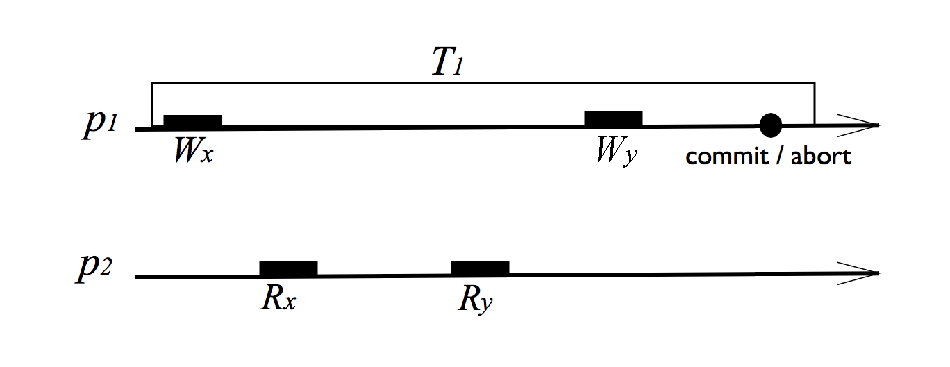
\includegraphics[width=80mm]{imgs/non_containment.eps}}
     \mbox{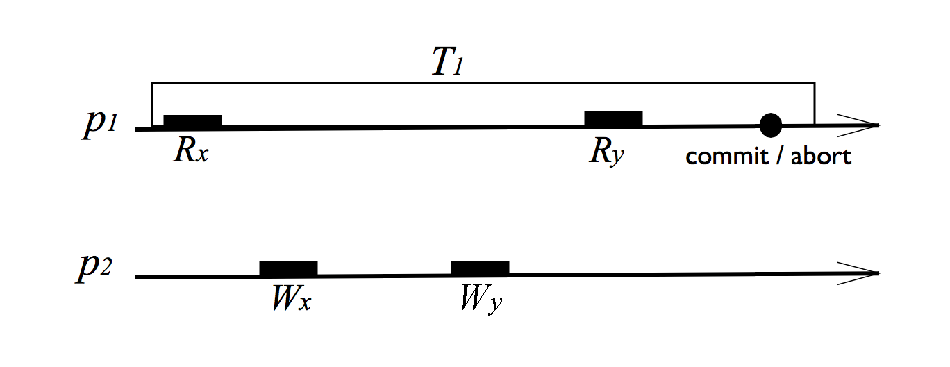
\includegraphics[width=80mm]{imgs/interference.eps}}
}
\caption{Left:  {\it Containment}  (operation $R_x$  should not  return the
    value written to $x$ inside the transaction). 
Right:  {\it  Non-Interference} (wile  it is still  executing, transaction
$T_1$ should not have access to the values that were written to $x$ and $y$
by process $p_2$).} 
\label{fig:int-nonc}
\end{figure*}


Non-interference violations can be caused  by the ABA problem. Consider the
case where a transaction $T$  
pertaining  to process  $p_1$  reads variable  $x$  through read  operation
$R_x$, and finds that it contains value  
$v_1$.  Before $T$  commits, and  after  $R_x$ has  completed, assume  that
another process $p_2$ modifies $x$  
by  writing value  $v_2$ to  it through  non-transactional  write operation
$W_{1x}$. Then, assume that either the  
same process  $p_2$ or a different process  $p_3$ write non-transactionally
value $v_1$ to $x$ through operation  
$W_{2x}$. In  this case, process  $p1$ should have  a means to  detect this
occurrence and transaction $T$ should  
not commit, given that otherwise, strong isolation would be violated. 


Non-interference for  a transaction  $T_1$ can also  be compromised  by 
interaction between non-transactional  
operations  and  another  transaction   $T_2$,  as  illustrated  in  Figure
\ref{fig:timent}. There, non-transactional operation  
$R_{2x}$  reads  what transaction  $T_2$  has  written  to shared  variable
$x$. Due to maintaining consistency, it is not  
possible  to find  a  correct serialization  order where  non-transactional
operation $W_y$ does not happen during the  
duration  of transaction $T_1$,  violating non-interference.  Therefore, in
order to preserve opacity, this situation would  
have to  be detected when  transaction $T_1$ attempts to  execute operation
$R_y$ and $T_1$ would have to be aborted. 
 

\begin{figure*}[h]
\centerline{
    \mbox{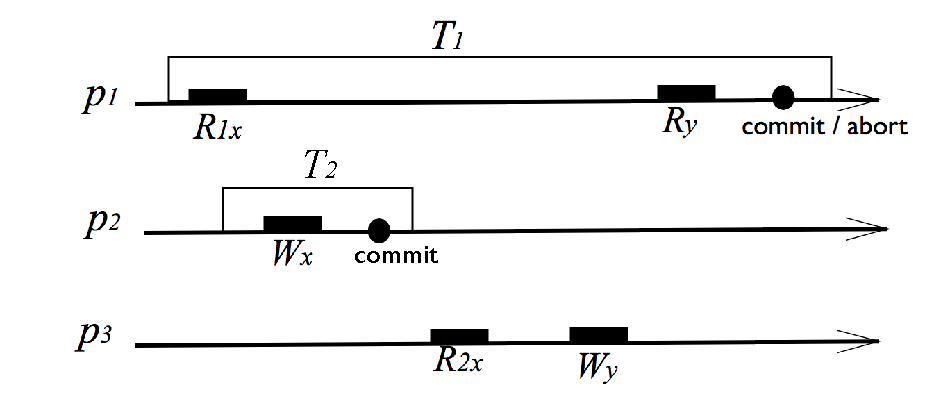
\includegraphics[width=80mm]{imgs/time_NT.eps}}
}
\caption{Transaction  $T_2$  and  non-transactional operations  of  process
$p_3$ interfere with transaction $T_1$.} 
\label{fig:timent}
\end{figure*}


\Xomit{%%%%
Many  TM algorithms,  and  so  also TL2,  already  trivially satisfy  strong
isolation and the characteristics that we consider that it implies,  
provided   that    shared   memory   is    exclusively   accessed   through
transactions. When shared memory is accessed through non-transactional  
operations also, the TM algorithm that is used has to be extended so that it
prevents the scenarios discussed above.  
} %%%\Xomit{%%%%


%========================================================================
\section{A brief presentation of TL2}
\label{sec:tl2}

This section presents the main  aspects of the  TM algorithm TL2  which  are  
used by the proposed algorithm. TL2 has been introduced by Dice, Shalev and Shavit 
in    2006    \cite{dice06}.   It does not allow for  non-transactional code.  We describe 
here the word-based version of TL2. In this  version it is considered that shared  memory 
is accessed in the granularity of  single  memory words.  For the sake of  clarity and without 
loss  of generality, the rest of the description  assumes that shared variables are the size of a 
memory word. Therefore,  the operations issued by a transaction are simply read and write operations.  



%---------------------------------------------------------------------
\subsection{Main features of TL2}
To control transaction synchronization, TL2 employs locks and 
logical dates. The variables  that a  transaction has to read form its read
set, while the variable it has to update, form its write set.  
A  transaction  first  has to  obtain  the  locks  that correspond  to  the
variables of its write set, before it can  
update them.  Conversely, a  transaction has to  check the logical dates  of the
variables in its read set, in  
order to  ensure that  the values  it has read  correspond to  a consistent
snapshot of shared memory.  


\paragraph{Locks}
TL2 locks  are stored in  a shared lock  table. Each shared memory  word is
mapped to a lock through a  
hash function\footnote{The  hash function is one-to-many,  resulting in one
lock covering several shared  
memory locations. This  partitions the memory into  so-called stripes.}. A
lock is a memory word where  
one of the  bits acts as lock  bit, indicating whether the lock  is free or
not. The rest of the bits form the  
logical date field.  The logical date of the lock  also serves as the 
logical date of the
memory  locations that  the lock  maps to.  Whenever a  shared  variable is
modified, its logical date is also updated. Due to the way the  
logical dates are assigned, they increment monotonically. 

\paragraph{Update vs read-only transactions}
TL2  makes  the  distinction  between  update  transactions  and  read-only
transactions. A {\it read-only} 
transaction consists  of a  begin phase and  an operation phase.  
An {\it update}  transaction consists  
of a  begin phase,  an operation phase,  and a  commit phase. In  an update
transaction, the operation  
phase will contain write operations to shared variables as well as possibly
read operations, while  
in a  read-only transaction, it  will solely contain read  operations. 

Read
operations in TL2 are {\it invisible},  
meaning  that when  a  transaction reads  a  shared variable,  there is  no
indication of that fact towards  
other transactions.  Write operations are  {\it deferred}, 
meaning that  TL2 does not perform the updates  
as soon as  it {}``encounters'' the shared  variables that  it has to write
to (i.e., during the operation  
phase). Instead, the updates it has to perform are logged into a local list
(also called  redo log) and   are  applied  to the shared  memory only once
the transaction is certain  to commit (i.e. which occurs  during the
commit phase). 


\paragraph{Logical time}
In order to implement logical time, TL2 employs an integer logical 
clock denoted  
$\mathit{GVC}$. Th? $\mathit{GVC}$ is incremented by update 
transactions when they attempt to commit. When it starts up, 
a transaction reads the current value of 
the $\mathit{GVC}$ into a local variable called $\mathit{rv}$. When a 
transaction attempts to commit, it performs an increment-and-fetch on 
$\mathit{GVC}$, and stores the 
return value in a local variable called $\mathit{wv}$
(which can be seen as a write version number  or a version timestamp). 
Should the transaction commit, it will write its $\mathit{wv}$ in the 
logical date field 
of all shared variables in its write set. 

Timestamping with logical dates facilitates read set validation for a 
transaction. 
When the read set of a transaction is 
not valid,  the transaction  cannot commit. The  read set of  a transaction
$T_A$ will be  invalidated  
if another,  concurrent transaction $T_B$ modifies shared  variable $x$ and
commits, after $T_A$  
has read $x$  but while $T_A$ is  still active. In TL2, it  can be detected
that a transaction{}'s read  
set is valid if the logical date of every  item on the read set is less 
than the
transaction{}'s $\mathit{rv}$  value. If, on the  contrary, the logical 
date of a read set  item is larger than
the $\mathit{rv}$ of the transaction,  
then this  indicates that,  in the meanwhile,  a concurrent  transaction has
performed  an   increment-and-fetch    of   $\mathit{GVC}$,   updated   the
item  and  committed,  by  writing  the  new 
$\mathit{GVC}$ value into the item{}'s  logical date field.



%========================================================================
\subsection{Inside a TL2 transaction}

\paragraph{Begin of a transaction}
When a  transaction starts  up, it  reads the current  value of  the $\mathit{GVC}$ 
and stores it into  
its local  $\mathit{rv}$ variable. A transaction  has to keep  track of the
variables in its read set and their  
versions, as well as the variables in  its write set and values that it has
to write to them. Therefore, it  
implements the  read and  write set  as local lists,  which will  be filled
during the transaction execution.  
These data structures are also initialized at start-up.

\paragraph{TL2 write}
When a transaction  has to update shared variable $x$,  it creates an entry
for it in its local write set list  
and there, it  stores $x${}'s address and the value that  has to be written
to it.  

\paragraph{TL2 read}
When  a transaction has  to read  shared variable  $x$, then,  if it  is an
update transaction, it first explores  
its local write set list in order to check whether $x$ is already contained
there. Should this be the case,  
then, in order to preserve consistency,  the value that is contained in the
write set list will be returned for  
the variable.  If the  update transaction doesn{}'t  find $x$ in  the write
set, then it proceeds as a read-only   transaction would proceed. 

Before and after reading $x${}'s value, a read-only transaction samples the
lock bit and the lock version  
corresponding to $x$. If the lock version is different before and after the
read or if the lock bit is set, then  
the transaction aborts, given that it has just detected a concurrent update
of $x$ which invalidates its read  
set.  If this  procedure, also  referred  to as  post-validation, does  not
result in aborting, then the operation can   
return the value that it has read  for $x$. If the transaction is an update
transaction, then, before returning the  
value, it  creates an entry for  $x$ in its  local read set list,  where it
stores the memory address of $x$.  

\paragraph{Attempt to commit}
After  having executed  all its  read and/or  write operations  in  the way
described before, a transaction attempts  
to commit. If  it is a read-only transaction and it  has reached this point
(i.e., has not been aborted during some  
read operation), then the post-validation that is performed after each read
has ensured that the values it has  
read for the  variables in its read set,  constitutes a consistent snapshot
of memory. Therefore, the read-only  
transaction  is considered  committed without  having to  take  any further
explicit action. 

On the contrary, an update  transaction has to explicitly verify whether it
can commit and explicitly make its  
commit  visible  to  the rest  of  transactions.  In  order to  update  the
variables in its write set, the transaction first  
has to  {}``obtain ownership'' for  them, i.e., lock  them, it then  has to
validate its read set, in order to ensure that  
by committing, it will not violate  consistency, and then it has to perform
the updates and release the locks it  
holds. 

\paragraph{Lock acquisition and $\mathit{GVC}$ increment} 
For  every item  in  the  transaction{}'s write  set,  bounded spinning  is
performed on the corresponding lock in order  
to  obtain  it.  If the  lock  acquisition  for  an  item fails,  then  the
transaction aborts. If, however, all locks are acquired  
successfully,   then  the   transaction  performs   increment-and-fetch  on
$\mathit{GVC}$ and stores the return value in  
local variable $\mathit{wv}$. This value of $\mathit{wv}$ will be stored as
the new version of the variables in the  
transaction's write set, if the transaction does not abort.

\paragraph{Validation of the read set}
In order  to determine whether the  transaction has to abort,  a final read
set validation takes place. During this  
validation, it  is verified  for all  items of the  read set  whether their
current version is still less that the transaction's  
read version, $\mathit{rv}$, as well as whether the items are not locked by
a different transaction. If it is detected  
that this is not the case  for any item, the transaction aborts. Otherwise,
the transaction can perform the intended  
updates. Read  set validation  is not necessary  in the special  case where
$\mathit{rv}$+1 = $\mathit{wv}$, given  
that this would  guarantee that no concurrent transaction  has executed and
possibly modified items of the read   set in the meanwhile.

\paragraph{Deferred updates and lock release}
The   address  and   update  value   for  each   shared  variable   in  the
transaction{}'s write set is stored in a corresponding  
entry  in the  transaction{}'s local  write set  list. Therefore,  for each
write set list entry, the update value is stored in the  
corresponding memory address. The  locks are released by atomically writing
the value of $\mathit{wv}$ to their lock  
version field  while clearing the lock bit. 




%========================================================================
\section{Implementing terminating strong  isolation}
\label{sec:protocol}

A traditional  solution to  the problem of  ensuring isolation   in the
presence of  non-transactional code consists in using  locks: Each shared
variable would then  
be associated with a lock and both transactions as well as non-transactional 
operations would have to acquire the lock before accessing the variable. In
order  to achieve strong isolation,  transactions would have to acquire the
locks of the  variables both in their read and in their write set.

Locks are already used  in TM algorithms - such as TL2  itself - where it is
however     assumed   that  shared   memory   is   only  accessed   through
transactions. The use  of locks  in a TM algorithm  entails blocking and may
even lead a process to starvation. However,  
it can be argued that  these characteristics are acceptable, given that the
programmer  accepts the fact that a  transaction has a duration and that it
may  even  fail: The  fact  that   there is  always  a  possibility that  a
transaction will abort means that the eventuality of  
failure to complete is an integral part of the transaction concept.  

On  the contrary,  when it  comes to  read or  write accesses  to  a shared
variable, a  non-transactional operation is  understood  as an
event  that  happens   atomically  and   completes.  Unfortunately   strong
isolation  implemented with  locks  entails the blocking  
of non-transactional read and write operations.

Given that this approach would be rather counter-intuitive for the 
programmer (as well as possibly detrimental for program efficiency), 
the   algorithm presented  in this  section  provides  a solution  for adding
strong isolation which does not based on locks for the execution 
of non-transactional  operations. This  algorithm builds on  the base  of TM
algorithm  TL2 and  extends it in  order to account for  non-transactional 
operations. While read   and write operations that appear inside a 
transaction follow the original TL2 algorithm rather closely (commit-time lock 
acquisition, write-back and validation of the  read set), 
the proposed algorithm 
specifies specific non-transactional read and  write operations 
that are to be used 
by the programmer, substituting conventional read and write operations. 
In the following sections, the memory setup, special data structures 
and operations will be explained.


%===================================================================
\subsection{Memory setup and data structures}


\paragraph{Memory setup}
The underlying memory system is made up of atomic read/write registers. 
Moroever some of them can also be accessed by the the following two 
operations. The operation denoted 
${\sf Fetch\&increment}()$ atomically adds one to the register and 
returns its previous value. 
 The operation denoted 
${\sf C\&S}()$ (for compare and swap) is a conditional write. 
${\sf C\&S}(x,a,b)$ writes $b$ into $x$ iff $x=a$. In that case it 
returns $\mathit{true}$. Otherwise it returns  $\mathit{false}$. 


The proposed TL2 extension assumes that the
variables  are  of  types and  values  that  can  be   stored in  a  memory
word. This assumption aids in the clarity of the algorithm description  
but it  is also  justified by the  fact that  the algorithm extends  TL2, an
algorithm that is   designed to be word-based. 

As in TL2,  the variable $\mathit{GVC}$
acts as  global  clock  which  is incremented  by update transactions.
 Apart from a global   notion of ``time'', there exists also
a local one, and therefore, each process maintains a local  
variable denoted $\mathit{time}$,  which is used in order to keep  
track of when, with
respect to the $\mathit{GVC}$, a non-transactional operation 
or a transaction was last performed by
the  process.
This variable is then used during non-transactional operations to ensure
the linearization of operations is not violated.
Each  process's  $\mathit{time}$   variable is   
therefore incremented
both during transactional and non-transactional operations.
Like TL2, update  transactions are assigned a logical time by
performing an increment-and-fetch
on  $\mathit{GVC}$, in this algorithm this value is also used to set the
value of the $\mathit{time}$ variable.  As  will  be explained  in  detail  later  on,
non-transactional operations update  
their process's $\mathit{time}$ variable either by  assigning it the value of 
the $\mathit{GVC}$, or by assigning it the  
logical date of a shared variable that they are accessing.

In TL2 a  shared array of locks is maintained and each
shared memory word  
is associated with a lock in this array. Given this, a memory
word directly contains  
the value of the variable that  is stored in it.
Instead, the algorithm presented here, uses
a  different memory setup that does not require a lock array, but does requires
an extra level of indirection when loading and storing values in memory.
Instead of storing a value of a variable directly to a memory word,
each  write  operation  on   variable  $\mathit{var}$,   transactional  or
non-transactional, creates an algorithm-specific data  
structure where  it stores  the value to  be written to  $\mathit{var}$, as
well as necessary meta-data.

Instead of locking each location in the write set during the commit operation like TL2, this algorithm
performs a compare and swap to each location setting the value of the word to point
a structure from the transaction's write set, effectively locking the location.
This process is described in detail later in this document.

\paragraph{T-record  and NT-record}
The  algorithm-specific  data structures  are shared  and  can be  of 
either  two  kinds, which will be referred   to as T-records and NT-records. 
A T-record is created by a transactional write operation while an 
NT-record is created by a  non-transactional write operation. A memory word
that is used to store  
variable $\mathit{var}$ at address $\mathit{addr}$ will then contain a pointer to a  
record of either of the  aforementioned types and within this structure
the actual value for  $\mathit{var}$ is stored as a field. 
This  is illustrated in Figure  \ref{fig:mem_setup}.

\begin{figure*}[h]
\centerline{
    \mbox{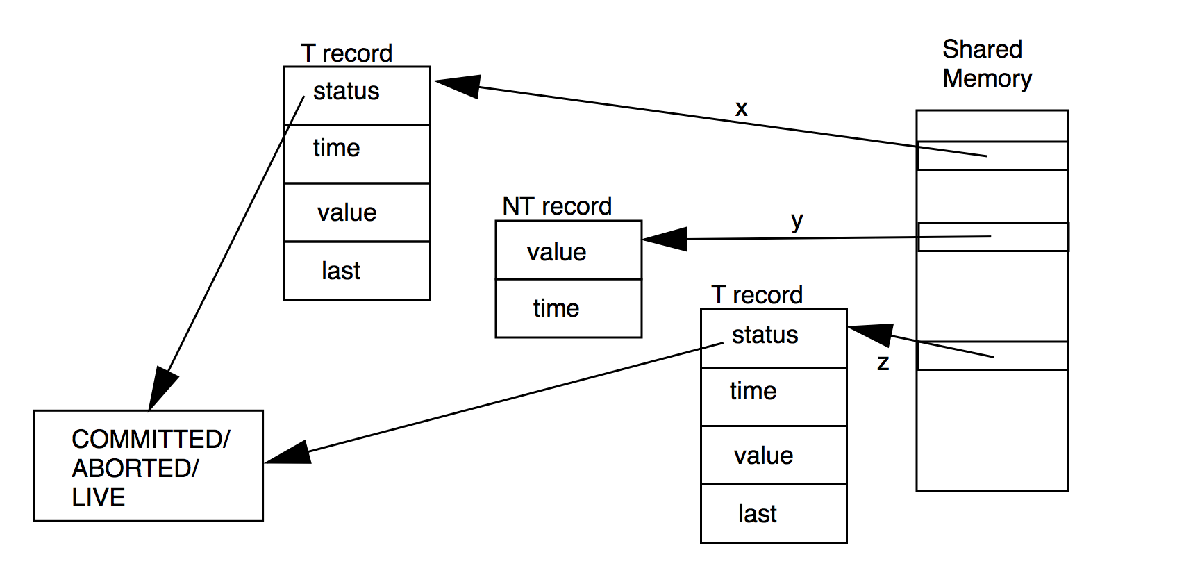
\includegraphics[width=100mm]{imgs/mem_setup_single.eps}}
}
\caption{The memory setup and the data structures that are used by the 
algorithm.}
\label{fig:mem_setup}
\end{figure*}

New T-records are created during the transactional write operations.
Then during
the commit operation the pointer stored at $\mathit{addr}$ is updated to point to this new T-record.
During NT-write operations new NT-records are created and the pointer at $\mathit{addr}$
is updated to point to the records.

When a read operation - be it transactional or non-transactional - accesses 
a shared variable it cannot know beforehand what type of record it will find 
on the list. Therefore, it can be seen in the algorithm listings, that whenever 
a record from the list is accessed, 
the operation checks its type, i.e., it checks 
whether it is a T-record or an NT-record (for example, line \ref{A02} in Figure 
\ref{fig:ntops} contains such a check. A T-record is {}``of type T'', while an 
NT-record is {}``of type NT''). 


\paragraph{T-record}
A T-record is a structure containing the following fields.
\begin{itemize}
\vspace{-0.1cm}
\item[$\mathit{status}$]
This  field  indicates  the  state  of the  transaction  that  created  the
T-record. The  
state can either be LIVE, COMMITTED or ABORTED.
The state is initially set to LIVE and is not set to COMMITTED until during the commit operation when 
all locations of the transaction's write set have been set to point to the transaction's T-records
and the transaction has validated its read set.
What is important to recognize is that during the commit operation, after a transaction has set some location to point to a T-record
of this transaction, and before the transactions status has been set to COMMITTED or ABORTED, the transaction has effectively
taken the lock on this location.
Like in TL2, any concurrent transaction that reads the location and sees that it is locked ($\mathit{status} = $ LIVE) will
abort itself.

Since a transaction can write to multiple locations, the $\mathit{status}$ field
does not directly store the state, instead it contains a
pointer to a memory location containing the state specific to a single transaction.
Therefore the $\mathit{status}$ field of each T-record created by the same transaction will point to the same location.
This ensures that any change to the transaction's state is immediately recognized at each record.
\vspace{-0.2cm}
\item[$\mathit{time}$]
The  $\mathit{time}$  field of  a T-record  contains the  
value of  the $\mathit{GVC}$  at  the  moment the  record  was 
inserted  into the  list of   records.
This is similar to the logical time values of TL2 that are stored in the lock array.
\vspace{-0.2cm}
\item[$\mathit{value}$]
This field contains the value that is meant to be written to the chosen 
memory location.
\vspace{-0.2cm}
\item[$\mathit{last}$]
As previously mentioned, during the commit operation, locations are updated to point
to the committing transaction's T-records, effectively locking the location, but also overwriting the previous value
that was stored in this location.
Like in TL2, validation is performed after locking the write locations, which might cause the transaction to abort.
In the case of the abort, the previous value of the location needs to be available for future reads.
In order to account for this, the $\mathit{last}$ field of a T-record
stores the previous value of this location before this T-record was pointed to.

\end{itemize}


\paragraph{NT-record}
An NT-record is a structure containing the following fields.
\begin{itemize}
\vspace{-0.1cm}
\item[$\mathit{value}$]
This field contains the value that is meant to be written to the chosen 
memory location.
\vspace{-0.2cm}
\item[$\mathit{time}$]
As in the case of T-records, the $\mathit{time}$ field of NT-records 
also stores the value 
of the $\mathit{GVC}$ when the write took place. This field is 
used to avoid inconsistencies such as the ones illustrated by Figure 
\ref{fig:timent}. 
\end{itemize}

Using these control data, the most  recent valid value  of a variable  can be
determined.  Should the item be of type NT-record,
then it's $\mathit{value}$ field contains the most  
recent valid value  of the variable. On the other hand,  should the item
 be a  T-record, then if the $\mathit{status}$ field of
the record is equal to COMMITTED,  
the $\mathit{value}$ field represents the current value of the variable. Otherwise, the
$\mathit{last}$ field contains the current value.

\paragraph{Transactional Read and Write Sets}
Like TL2, read only transactions do not use read sets while update transactions do.
The read set is made up of a set of tuples for each location read, $\tuple{\mathit{addr, value}}$
where $\mathit{addr}$ is the address of the location read and $\mathit{value}$ is the value
read from the location.
The write set is also made up of tuples for each location written by the transaction,
$\tuple{\mathit{addr, item}}$ where $\mathit{addr}$ is the location to be written
and $\mathit{item}$ is a T-record that will be pointed to during the commit operation.

\subsubsection{Discussion}
One advantage of the TL2 algorithm is in its memory layout.
This is because reads and writes happen directly to memory (without indirection)
and the main amount of additional memory that is used is in the lock array.
Unfortunately this algorithm breaks that and requires an additional level of indirection
as well as additional memory per location.
These additional requirements can be an acceptable trade-off given that they are only
needed for memory that will shared between transactions.
Still, in the appendix we present two variations of the algorithm that trade
off different memory schemes for different costs to the transactional and
non-transactional operations.

***Note: In order to save more memory, the time variable of the T-record can be combined
with the status variable.

%====================================================================

\subsection{Description of the algorithm}

The main goal of the algorithm is to provide strong isolation 
in such a way that  the non-transactional  operations are never blocked. 
In order  to achieve this,  the algorithm delegates most of  
concurrency   control   and  consistency   checks   to  the   transactional
code. Non-transactional  
operations access and modify  memory  locations without waiting for concurrent transactions
 and it is mainly up to transactions accessing the same location to
do it in a way that ensures safe  
concurrency - and to abort if this  is not possible.  As a
result, this algorithm gives high  priority   to non-transactional code. 

Given the particular memory arrangement  that the algorithm uses, two helper
procedures are used  to perform load  or store. They are
presented  in  Figure  \ref{fig:aux}.\footnote{The following  notation  is
used. If $pt$ is a pointer, $pt\downarrow$ is the object pointed to by $pt$. 
if $aa$ is an object, $\uparrow aa$ is a pointer to $aa$. Hence 
$((\uparrow aa)\downarrow =aa$ and $ \uparrow(pt \downarrow)=pt$.}


\begin{figure}[htb]
\centering{ \fbox{
\begin{minipage}[t]{150mm}
\footnotesize 
\renewcommand{\baselinestretch}{2.5} 
%\resetline
%\setcounter{linecounter}{200}
\begin{tabbing}
aaaaaaa\=aa\=aaaaa\=aa\=aa\=\kill %~\\


{\bf operation} ${\sf load}(addr)$ {\bf is}  
%\line{help1} \> 
${\sf return} (addr \downarrow)$ {\bf end operation}.  \\
\\
{\bf operation} ${\sf store}(addr, value)$ {\bf is} 
%\line{help2} \> 
$(addr \downarrow) \gets value$ {\bf end operation}.

\end{tabbing}
\normalsize
\end{minipage}
}
\caption{Helper operations for load and store operations.}
\label{fig:aux}
}
\end{figure}


In the following operation descriptions, we assume that the shared variable
that  is   accessed  by  transactional or  non-transactional operations  is
denoted $\mathit{var}$, and   
it is allocated the memory word at address $\mathit{addr}$.



%=====================================================================
\subsection{Non-transactional operations}
In  order  to  comply  with  the  algorithm a  programmer  has  to  use  the
algorithm-specific   read  and write  operations when a  variable has  to be
accessed outside of a transaction.  This can also be applied by a complier.
Algorithms for these operations is presented in Figure \ref{fig:ntops}. 

\begin{figure}[htb]
\centering{ \fbox{
\begin{minipage}[t]{150mm}
\footnotesize 
\renewcommand{\baselinestretch}{2.5} 
%\resetline
%\setcounter{linecounter}{200}
\begin{tabbing}
aaaaaaa\=aa\=aaaaa\=aa\=aa\=\kill %~\\


{\bf operation}  ${\sf non\_transactional\_read}(\mathit{addr})$ {\bf is}\\
\line{A01} \> $\mathit{tmp} \gets {\sf load}(\mathit{addr})$; \\ 
\line{A02} \> {\bf if} $( ~\mathit{tmp}$ is of type T $ \cap \mathit{tmp.status} \neq$ COMMITTED ) \\
\line{A03}  \>\>  {\bf then if}  $(\mathit{tmp.time}  \leq \mathit{time}  \wedge  \mathit{tmp.status} = $ LIVE) \\
\line{A04} \>\>\>\> {\bf then} \=${\sf \mathit{C\&S}}$($tmp.status$, LIVE, ABORTED) {\bf end if}; \\
%\line{A05} \>\> {\bf end if} \\
\line{A06} \>\>\> {\bf if} ($tmp.status \neq $ COMMITTED)  \\
\line{A07} \>\>\>\> {\bf then} $\mathit{value} \gets \mathit{tmp.last}$ \\
\line{A08} \>\>\>\> {\bf else} $\mathit{value} \gets \mathit{tmp.value}$ \\
\line{A05} \>\>\> {\bf end if}; \\
\line{A09} \>\> {\bf else} $\mathit{value} \gets \mathit{tmp.value}$ \\
\line{A09A} \> {\bf end if}; \\
\line{A10} \> $\mathit{time} \gets {\sf max}(\mathit{time}, \mathit{tmp.time})$ \\
\line{A11} \> {\bf if} ($\mathit{time} = \infty$) {\bf then} $\mathit{time} = \mathit{GCV}$ {\bf end if}; \\
\line{A12} \> ${\sf return}$ ($\mathit{value}$) \\
{\bf end operation}. \\
\\
{\bf operation}  ${\sf non\_transactional\_write}(\mathit{addr, value})$ {\bf is}\\
\line{B01} \> allocate new variable $\mathit{next\_write}$ of type NT; \\
\line{B02} \> $\mathit{next\_write} \gets \mathit{(addr, value, \infty)}$; \\
\line{B03} \> ${\sf store}(\mathit{addr, next\_write})$ \\
\line{B04} \> $\mathit{time} \gets \mathit{GVC}$; \\
\line{B05} \> $\mathit{next\_write.time} \gets \mathit{time}$; \\
{\bf end operation}.

\end{tabbing}
\normalsize
\end{minipage}
}
\caption{Non-transactional operations for reading and writing a variable.}
\label{fig:ntops}
}
\end{figure}

\paragraph{Non-transactional read}
The   operation  ${\sf   non\_transactional\_read()}$  is   used   to  read,
when not in a transaction, the value stored at
$\mathit{addr}$.
The  operation first  dereferences  the pointer  stored at  $\mathit{addr}$
(line \ref{A01}).
If the item is a T-record that was created by a 
transaction which  has not yet  committed then the $\mathit{value}$ field
cannot be immediately be read as the transaction might abort.
If the current process has read a value that is more recent then the transaction
(meaning the process's $\mathit{time}$ field is greater or equal to the T-records
$\mathit{time}$, line \ref{A03}) then the transaction must be directed to abort (line \ref{A04})
in order to insure containment? is not violated.

From a T-record with a transaction that is not committed, the value from the $\mathit{last}$
field is stored to a local variable (line \ref{A07}) and will be returned on operation completion.
Otherwise the $\mathit{value}$ field of the T or NT-record is used (line \ref{A08}).

Once  the correct value  has been  found  and stored  in local  variable 
$\mathit{value}$, the local $\mathit{time}$   
variable  is updated  (lines \ref{A10}-\ref{A11}).  The updated  $\mathit{time}$
value is used by non-transactional operations and is necessary in order to allow 
the detection of consistency 
violations such as the one illustrated by Figure \ref{fig:timent}. 
By advancing the value of $\mathit{time}$ 
through a non-transactional read operation, 
the serialization order of this read operation with 
respect to transactional or non-transactional operations 
that it read from is reflected.

The process local variable $\mathit{time}$ is advanced to 
the maximal 
value among its current 
value and the logical date of the T or NT-record whose value was read.
Finally if $\mathit{time}$ was set to $\infty$ on line \ref{A10}, then it is updated
to the $\mathit{GCV}$ on line \ref{A11}.
Once these book-keeping 
operations are finished, the local variable $\mathit{value}$
is returned (line \ref{A12}).

\paragraph{Non-transactional write}
The operation ${\sf non\_transactional\_write()}$ is used to write to 
a shared variable $\mathit{var}$ 
by non-transactional code.
The operation takes as input the address of the shared variable as well as the 
value that has to be written to it as arguments.
This operation  
creates a  new  NT-record  (line  \ref{B01}),  fills  in  its  fields  (line
\ref{B02})  and 
changes the pointer stored in $\mathit{addr}$ so that it references the 
new record it has created  (line \ref{B03}).
Unlike update transactions, non-transactional writes do not increment
the global clock variable $\mathit{GCV}$.
Instead they just read $\mathit{GCV}$ and set the NT-record's time value as well as
the process local $\mathit{time}$ to the value read (line \ref{B04} and \ref{B05}).
Since the $\mathit{GCV}$ is not incremented, several NT-records might have the same
$\mathit{time}$ value as some transaction.
When such a situation is recognized where a live transaction has the same time value
as an NT-record the transaction is aborted (if during an NT-read operation,
line \ref{A04}) or read set validation is performed (if during a transactional
read operation, line \ref{C05} of figure \ref{fig:tops}).
This is done in order to prevent consistency violations such as the one shown 
in Figure \ref{fig:timent}.


%==================================================================
\subsection{Transactional read and write operations}

The transactional operations for performing reads and writes are 
presented in Figure \ref{fig:tops}. 

\paragraph{Transactional read}

The operation ${\sf  transactional\_read()}$ receives $\mathit{addr}$ as an
input argument. It starts by checking  
whether the  desired variable already  exists in the  transaction{}'s write
set, in which  
case  the   value  stored  in  the   write  set  will   be  returned  (line
\ref{C01}). If the variable is not contained  
in  the write  set, the  pointer in  $\mathit{addr}$ is  dereferenced (line
\ref{C02}) and set to $\mathit{tmp}$. Once the structure pointed to is detected to be a T or NT-record
some checks are then performed in order to ensure correctness.

In the case that $\mathit{tmp}$ is a T-record the operation must check to see
if the status of the transaction for this record is still LIVE and if it is
the current transaction is aborted (line \ref{C10}).
This is similar to TL2 aborting the transaction when a locked location is found.
Next, the T-record's $\mathit{time}$ field is checked, and (similar to TL2) if it 
greater then the process's local $\mathit{rv}$ value the transaction must abort 
(line \ref{C12}).
If this succeeds without aborting then the local variable $\mathit{value}$
is set depending on the stats of the transaction that created the T-record (line \ref{C10}-\ref{C11}).


In case $\mathit{tmp}$ is an 
NT-record (line \ref{C03}), the operation
checks whether the value of the $\mathit{time}$ field is
greater or equal to the process local $\mathit{rv}$ value.
If it is, then this write has possibly occured after the start of this
transaction and there are several possibilities.
In the case of a read only transaction, the transaction
is aborted and restarted as an update transaction (line \ref{C06}),
while an update transaction must perform validation, ensuring
that none of the values it has read have been updated (line \ref{C05}).
Finally local variable $\mathit{value}$ is set to be the value
of the $\mathit{value}$ field of the $\mathit{tmp}$ (line \ref{C07}).

It should be noted that the reason why the checks are performed differently
for NT-records and T-records is because the NT-write operations do not
update the global clock value while update transaction do.
This means that the checks must be more conservative in order to ensure correctness.
If performing per value validation or restarting the transaction as an update transaction
is found to be too expensive, a third possibility would be to just increment the global
clock, then restart the transaction as normal.


Finally to finish the read operation, the $\tuple{\mathit{addr, value}}$
is added to the read set if the transaction is an update transaction (line \ref{C14}),
and the value of the local variable $\mathit{value}$  is returned.

\begin{figure} %[htb]
\centering{ \fbox{
\begin{minipage}[t]{150mm}
\footnotesize 
\renewcommand{\baselinestretch}{2.5} 
%\resetline
%\setcounter{linecounter}{200}
\begin{tabbing}
aaaaaaa\=aa\=aaaaa\=aa\=aa\=\kill %~\\


{\bf operation}  ${\sf transactional\_read}(\mathit{addr})$ {\bf is}\\
\line{C01} \> {\bf if} $\mathit{addr} \in \mathit{ws}$  {\bf then} ${\sf return}$ ($\mathit{item.value}$ from $\mathit{addr}$ in $\mathit{ws}$)  {\bf end if}; \\
\line{C02} \> $\mathit{tmp} \gets {\sf load}(\mathit{addr})$; \\

\line{C03} \> {\bf if} ($\mathit{tmp}$ is of type NT)   \\
\line{C04} \>\> {\bf then} {\bf if} ($\mathit{tmp.time} >= \mathit{rv}$) \\
\> \% Do validation to prevent abort due to a non-transactional write \\
\line{C05} \>\>\> {\bf then if} this is an update transaction {\bf then} ${\sf validate\_by\_value}$() \\
\line{C06} \>\>\>\>\> {\bf else} ${\sf abort}$() and restart as an update transaction {\bf end if}; \\

\line{C06A} \>\>\> {\bf end if}; \\
\line{C07} \>\>\> $\mathit{value} \gets \mathit{tmp.value}$; \\

\line{C08} \>\> {\bf else} \\
\line{C09} \>\>\> {\bf if} ($(\mathit{status} \gets \mathit{tmp.status}) \neq$ COMMITTED $)$ \\
\line{C10} \>\>\>\> {\bf then if} ($\mathit{status} =$ LIVE) {\bf then} ${\sf abort}()$  {\bf else} $\mathit{value} \gets \mathit{tmp.last}$ {\bf end if}; \\
\line{C11} \>\>\>\> {\bf else} $\mathit{value} \gets \mathit{tmp.value}$ \\
\line{C11A} \>\>\> {\bf end if}; \\
\line{C12} \>\>\> {\bf if} $(\mathit{tmp.time} > \mathit{rv})$ {\bf then} ${\sf abort}()$ {\bf end if}; \\
\line{C13} \> {\bf end if}; \\

\line{C14} \> {\bf if} this is an update transaction 
                        {\bf then} add $\tuple{\mathit{addr,value}}$ to $\mathit{rs}$ {\bf end if}; \\
\line{C15} \> ${\sf return}$ ($\mathit{value}$) \\
{\bf end operation}. \\
\\
{\bf operation}  ${\sf transactional\_write}(\mathit{addr, value})$ {\bf is}\\
\line{D01} \> {\bf if} $\mathit{addr} \not\in \mathit{ws}$  \\
\line{D02} \>\> {\bf then} \> allocate a new variable $item$ of type $T$; \\
\line{D03} \>\>\> $\mathit{item}  \gets (\mathit{value, status, \infty})$; 
                   $\mathit{ws} \gets \mathit{ws} \cup \tuple{\mathit{addr, item}}$; \\
\line{D04} \>\> {\bf else} \> set $\mathit{item.value}$ with $\mathit{addr}$ in $\mathit{ws}$ to $\mathit{value}$ \\
\line{D05} \> {\bf end if}; \\
{\bf end operation}.
\end{tabbing}
\normalsize
\end{minipage}
}
\caption{Transactional operations for reading and writing a variable.}
\label{fig:tops}
}
\end{figure}

\paragraph{Transactional write}
The transactional write operations in this algorithm are performed by 
operation ${\sf transactional\_write()}$. 
It receives $\mathit{addr}$ as input value, as well as the value 
to be written to $\mathit{var}$. As  TL2, the algorithm 
performs commit-time updates of the variables it writes to. 
For this reason, the transactional write  
operation simply creates a T-record and fills in some of its 
fields (lines \ref{D02} - \ref{D03}) and also 
adds it to the transaction{}'s write set.
However, in the case that a T-record corresponding to $\mathit{addr}$  was
already present in  the write set, the
$\mathit{value}$ field of the corresponding  
T-record is simply updated (line \ref{D04}).


\paragraph{Begin and end of a transaction} 
Book-ending a transaction are operation ${\sf begin\_transaction()}$ 
and operation ${\sf try\_to\_commit()}$, which are 
presented in Figure \ref{fig:tbc}. ${\sf begin\_transaction()}$ 
initializes local variables that will be necessary 
for the execution of the transaction.
This includes $\mathit{rv}$
which is set to $\mathit{GCV}$ and like in TL2 is used during transactional
read to ensure correctness, 
as well as $\mathit{status}$ which is set to LIVE and the read and write sets
which are initialized as empty sets.
(lines \ref{START1}-\ref{START3}). 

\begin{figure} [htb]
\centering{ \fbox{
\begin{minipage}[t]{150mm}
\footnotesize 
\renewcommand{\baselinestretch}{2.5} 
%\resetline
%\setcounter{linecounter}{200}
\begin{tabbing}
aaaaaaa\=aa\=aaaaa\=aa\=aa\=\kill %~\\

{\bf operation}  ${\sf begin\_transaction}()$ {\bf is}\\
\line{START1} \> determine whether transaction is update transaction based on compiler/user input \\
\line{START2} \> $\mathit{rv} \gets \mathit{GVC}$; 
                 Allocate new variable $\mathit{status}$; \\
\line{START3} \> $\mathit{status} \gets $LIVE; \ $\mathit{ws} \gets \emptyset$; $\mathit{rs} \gets \emptyset$ \\
%\line{DA03} \> more??? \\
{\bf end operation}. \\
\\
{\bf operation}  ${\sf try\_to\_commit}()$ {\bf is}\\
\line{DA01} \> {\bf if} $(\mathit{ws} = \emptyset)$ {\bf then} ${\sf return}$ (COMMITTED) {\bf end if}; \\

\line{DA02} \> 
{\bf for each} $(\tuple{\mathit{addr, item}} \in \mathit{ws})$ {\bf do} \\

\line{DA03} \>\> $\mathit{tmp} \gets {\sf load}(\mathit{addr})$; \\


\line{DA04} \>\> {\bf if} 
   ($\mathit{tmp}$ is of type $T \wedge (\mathit{status} \gets \mathit{tmp.status}) \neq$ COMMITTED $)$  \\
\line{DA05} \>\>\> {\bf then if} ($\mathit{status} =$ LIVE) {\bf then} ${\sf abort}()$  {\bf else} $\mathit{item.last} \gets \mathit{tmp.last}$ {\bf end if}; \\
\line{DA06} \>\>\> {\bf else} $\mathit{item.last} \gets \mathit{tmp.value}$ \\
\line{DA06A} \>\> {\bf end if}; \\
\line{DA07} \>\> $\mathit{item.time} \gets \mathit{tmp.time}$; \\

\line{DA08} \>\> {\bf if} $(\neg {\sf \mathit{C\&S}}(\mathit{addr, tmp, item}))$ {\bf then} ${\sf abort}()$ {\bf end if}; \\
%\line{DA09} \>\>\> {\bf then} ${\sf abort}()$ \\
%\line{DA10} \>\> {\bf end if} \\

\line{DA11} \> {\bf end for}; \\

\line{DA12} \> $\mathit{time} \gets {\sf fetch\&increment}(\mathit{GVC})$; \\

\line{DA13} \> ${\sf validate\_by\_value}()$;  \\


\> \% Ensure the writes haven't been overwritten by non-transactional writes \\
\line{DA14} \> 
{\bf for each} ($\tuple{\mathit{addr, item}} \in \mathit{ws}$) {\bf do} \\
\line{DA15} \>\> $\mathit{item.time} \gets \mathit{time}$; \\
\line{DA16} \>\> {\bf if} $(\mathit{item} \neq load(\mathit{addr}))$  
                 {\bf then}  
                   ${\sf abort}()$ 
                {\bf end if}; \\

\line{DA17} \> {\bf end for}; \\
\line{DA18} \> {\bf if} ${\sf \mathit{C\&S}}$($\mathit{status}$, LIVE, COMMITTED) \\
\line{DA19} \>\> {\bf then} \> ${\sf return}$ (COMMITTED)\\
\line{DA20} \> \> {\bf else} \= ${\sf abort}()$ \\
\line{DA21} \> {\bf end if};  \\
{\bf end operation}.

\end{tabbing}
\normalsize
\end{minipage}
}
\caption{Transaction begin/commit.}
\label{fig:tbc}
}
\end{figure}

After  performing all  required read  and write  operations,  a transaction
tries to commit, using the operation  ${\sf try\_to\_commit()}$.
Similar to TL2, a ${\sf try\_to\_commit()}$ operation 
starts by trivially committing if the transaction was a read-only one 
(line \ref{DA01}) while
an update transaction must announce to concurrent operations what locations it will be updating
(the items in the write set).
However, the algorithm  differs 
here from TL2, given that 
it is faced with concurrently happening non-transactional operations
that do not rely on locks and never block. 
This, in turn, implies 
that even after acquiring the locks for all items in its write set, 
a transaction could be {}``outrun'' by 
a non-transactional operation that writes to one of those items
causing the transaction to be required to abort in order to ensure correctness. 
Therefore while TL2 locks items in its write set using a
lock array, this algorithm compare and swaps pointers directly to the T-records
in its write set (lines \ref{DA02}-\ref{DA11}).
By following these pointers concurrent operations can access directly the
$\mathit{status}$ variable of the transaction and abort the transaction
if necessary.
Given that the compare and swap operations overwrite the previous values
and that the transaction can still be aborted,
the previous value for a given location must be stored in the T-record
before the compare and swap is performed (lines \ref{DA05}-\ref{DA06}).
Like how transactions in TL2 abort themselves when they encounter a locked
location from its write set,
if while performing these compare and swaps if the transaction notices
that another LIVE transaction is updating this memory, it aborts itself
(line \ref{DA05}).

The operation then advances the $\mathit{GVC}$, taking the
new value of the clock as the logical time for this transaction (line \ref{DA12}).
Following this the read set of the transaction is validated for
correctness (line \ref{DA13}).
Once validation has been performed the operation must
ensure that non of its writes have been concurrently
overwritten by non-transactional operations (lines \ref{DA14}-\ref{DA17})
if so then the transaction aborts (line \ref{DA16}).
While performing this check the transaction updates the $\mathit{time}$
value of its T-records to the transactions logical time (line \ref{DA15}).

After having added all its write set items to the respective 
record lists for the corresponding variables 
and after having verified that its read sets are valid, the 
transaction can mark its updates as valid by 
changing its 
$\mathit{status}$ variable from LIVE to COMMITTED (line \ref{DA18}).
This is done using a compare and swap as there could be
a concurrent non-transactional operations trying to abort the transaction.  
If this succeeds then the transaction has successfully committed, otherwise
it must abort and restart.


\begin{figure} [htb]
\centering{ \fbox{
\begin{minipage}[t]{150mm}
\footnotesize 
\renewcommand{\baselinestretch}{2.5} 
%\resetline
%\setcounter{linecounter}{200}
\begin{tabbing}
aaaaaaa\=aa\=aaaaa\=aa\=aa\=\kill %~\\

{\bf operation} ${\sf validate\_by\_value}()$ {\bf is}\\
\line{H01} \> $\mathit{rv} \gets \mathit{GVC}$; \\
\line{H02} \> {\bf for each} $\tuple{\mathit{addr, value}}$ in $\mathit{rs}$ {\bf do} \\
\line{H03} \>\> $\mathit{tmp} \gets load(\mathit{addr})$; \\
\line{H04} \>\> {\bf if} ($\mathit{tmp}$ is of type T $ \wedge \mathit{tmp.status} \neq $ COMMITTED) \\
\line{H05} \>\>\> {\bf then if} ($\mathit{tmp.status} =$ LIVE $\wedge \mathit{item} \not \in \mathit{ws}$)
     {\bf then} ${\sf abort}()$ {\bf end if}; \\
\line{H06} \>\>\>\> $\mathit{new\_value} \gets \mathit{tmp.last}$; \\
\line{H07} \>\>\> {\bf else} $\mathit{new\_value} \gets \mathit{tmp.value}$ \\
\line{H07A} \>\> {\bf end if}; \\
\line{H08} \>\> {\bf if} $\mathit{new\_value} \neq \mathit{value}$
     {\bf then} ${\sf abort}()$ {\bf end if}; \\
\line{H09} \> {\bf end for}; \\
{\bf end operation}. \\
\\
{\bf operation} ${\sf abort}()$ {\bf is}\\
\line{AB01} \> $\mathit{status} \gets $ ABORTED; \\
\line{AB02} \> the transaction is aborted and restarted \\
%\line{H21} \> free items in $\mathit{ws}$, $\mathit{rs}$, and $\mathit{ntrs}$; \\
%\line{H22} \> jump to line \ref{START1} \\
{\bf end operation}. \\
\end{tabbing}
\normalsize
\end{minipage}
}
\caption{Transactional helper operations.}
\label{fig:helpers}
}
\end{figure}


\paragraph{Transactional helping operations} 
Apart from the basic operations for starting, committing, 
reading and writing, a transaction makes use of helper 
operations to perform aborts and validate the read set.
 Pseudo-code for this kind of helper operations 
is given in Figure \ref{fig:helpers}.

Operation ${\sf validate\_by\_value()}$ is an operation that performs 
validation of the $\mathit{rs}$ of a transaction. 
Validation fails 
will happen if any location in $\mathit{rs}$ is 
currently being updated by another transaction (line \ref{H05})
or has had its changed since it was first read by the transaction (line \ref{H08})
otherwise it succeeds.
The transaction is immediately aborted if validation fails (lines \ref{H05}, \ref{H08}).
Before the validation is performed the read version ($\mathit{rv}$) is updated
to be the current value of the global clock (line \ref{H01}).
This is done because the transaction is still valid at this time and a larger
clock value could prevent future validations and aborts.

When a transaction is aborted in the present algorithm, 
the status of the current transaction is set to ABORTED (line \ref{AB01}) and
it is immediately restarted as a new transaction.


%========================================================================

\section{Conclusion}
\label{sec:conclusions}
This paper has presented an algorithm that achieves non-blocking strong 
isolation  ``on top of'' a TM algorithm based on logical dates and locks, 
namely  TL2. 
In case of conflict of a transactional and a non-transactional
operation on a shared variable, this algorithm gives priority to 
the non-transactional operation, 
reasoning that while an eventual abort or restart is part of the 
specification of the transaction,
this is not the case for conventional read or write operations. 
Due to this priority mechanism, 
the proposed algorithm is   particularly appropriate  for environments 
in which processes do not rely heavily
on the use of transactions and where non-transactional memory 
accesses are dominant. In 
such environments, strong isolation is  provided for transactions, 
while conventional read and write operations execute with a small overhead.


\Xomit{%%%%%%%%%%%%%%
In order to implement this priority mechanism, 
the algorithm will often preemptively abort transactions 
on the sole suspicion that they might violate consistency, 
even though those transactions might have 
turned out to be acceptable. This results in an algorithm that 
is not permissive, in the intuitive sense of 
permissiveness \cite{Guerraoui:2008:PTM:1432291.1432313}. 
Future work would focus on creating 
a more permissive version of the algorithm as well as on 
examining the application of some of the 
algorithm principles to non-blocking TM algorithms in order 
to equip them with mechanisms that provide strong isolation.
}  %%%%%%%%%\Xomit{%%%%%%%%%%%%%%



%========================================================================
%\bibliographystyle{unsrt}
%\bibliography{biblio}


{\small 

\begin{thebibliography}{guerraoui08}


\bibitem{afek10}
 Afek Y.,  Avni H.,   Dice D. and  Shavit N.,
Efficient lock free privatization. 
{\it Proc.  14th Int'l conference on Principles of Distributed Systems 
(OPODIS'10)}, Springer-Verlag,  LNCS \#6490, pp. 333-347, 2010. 



\bibitem{CIR12} 
Crain T., Imb D. and Raynal M., 
Towards a Universal Construction for Transaction-based Multiprocess Programs.
{\it Proc. 13th Int'l Conference on Distributed Computing and Networking
(ICDCN'12)}, 
Springer Verlag LNCS \#7129, pp. 61-75, 2012. 



\bibitem{dice10}
Dice D., Matveev A. and  Shavit N.,
 Implicit privatization using private transactions. 
{\it Proc. Workshop on transactional memory (TRANSACT'10)}, 2010.




\bibitem{dice06}
Dice D., Shalev O. and Shavit N.,
Transactional Locking II.
{\em Proc. 20th Int'l Symposium on Distributed Computing (DISC'06)},
Springer-Verlag, LNCS \#4167, pp.~194-208, 2006.


\bibitem{guerraoui08}
Guerraoui R. and  Kapalka M.,  
 On the correctness of transactional memory. 
{\it  Proc. 13th ACM SIGPLAN Symposium on Principles and Practice of 
Parallel Programming (PPoPP '08)},  ACM Press, pp.  175-184, 2008.




\bibitem{harris06}
 Harris T.,  Larus J., and  Rajwar R., 
Transactional Memory, 
{\it 2nd edition, Synthesis Lectures on Computer Architecture},
Morgan \& Claypool Publishers,  2006.




\bibitem{herlihy93}
Herlihy M.  and Moss J.M.B,
 Transactional memory: architectural support for lock-free data structures, 
{\it Proc.  of the 20th annual Int'l Symposium on Computer Architecture 
(ISCA '93)}, ACM Press, pp. 289-300, 1993. 



\bibitem{IR09} 
Imb D. and Raynal M., 
A versatile   STM protocol with invisible read operations 
that satisfies  the  virtual world consistency condition.
{\it   16th  Colloquium   on  Structural   Information   and  Communication
Complexity  (SIROCCO'09)}, 
Springer Verlag LNCS   \#5869, pp. 266-280,  2009.


\bibitem{maessen07}
 Maessen J.-W.and Arvind M.,
 Store Atomicity for Transactional Memory. 
{\it Electronic  Notes  on Theoretical  Computer Science}, 
174(9):117-137, 2007.


\bibitem{blundell06}
 Martin M.,  Blundell C.  and E. Lewis E.,
 Subtleties of Transactional Memory Atomicity Semantics. 
{\it IEEE Computer Architecture  Letters},  5(2):  2006.


\bibitem{MS12}
Matveev A. and  Shavit N.,
Towards a Fully Pessimistic STM Model. 
{\it Proc. Workshop on transactional memory (TRANSACT'12)}, 2012.



\bibitem{P79}
Papadimitriou Ch.H., 
The Serializability of Concurrent Updates. 
{\it Journal of the ACM},  26(4):631-653, 1979. 


\bibitem{scott07}
 Scott M.L.,  Spear, M.F. Dalessandro L.  and  Marathe V.J..
 Delaunay Triangulation with Transactions and Barriers. 
{\it Proc.  10th IEEE Int'l Symposium on Workload Characterization (IISWC '07)},
 IEEE Computer Society, pp. 107-113, 2007.





\bibitem{shavit95}
 Shavit N. and  Touitou D.,
 Software transactional memory. 
Software Transactional Memory. 
{\it Distributed  Computing}, 10(2):99-116, 1997. 


\bibitem{shpeis07}
 Shpeisman T.,  Menon V.,  Adl-Tabatabai A.R.,  Balensiefer  S.,  Grossman D.,
 Hudson R.L., K Moore K.F.  and  Saha B., 
Enforcing isolation and ordering in STM. 
{\it ACM  SIGPLAN Noticers}, 42(6):78-88,  2007.





\bibitem{spear08}
Spear M.F.,  Dalessandro L.,  Marathe V.J. and  Scott M.L., 
Ordering-Based Semantics for Software Transactional Memory. 
{\it Proc  12th Int'l Conference on Principles of Distributed Systems 
(OPODIS '08)},  Springer-Verlag LNCS \#5401, pp. 275-294. 2008. 



\bibitem{spear07}
Spear M.F.,  Marathe V.J. Dalessandro L. and  Scott M.L., 
Privatization techniques for software transactional memory. 
{\it Proc. 26th  annual ACM symposium on Principles of Distributed Computing 
(PODC '07)}, . ACM press, pp.  338-339, 2007.



\end{thebibliography}

}

\appendix
\section{Version of algorithm that does not use NT-records}
This algorithm also provides wait-free NT read and write operations.
The difference is that NT-records are not used.
Instead NT values are read and written directly from memory.
By doing this, memory allocations are not needed in NT writes and NT reads have
one less level of indirection.

The cost of this is more frequent validations required in transactions when conflicts with NT writes occur.
This algorithm is shown in Figures \ref{fig:ntops2}-\ref{fig:tbc2}.


\begin{figure}[htb]
\centering{ \fbox{
\begin{minipage}[t]{150mm}
\footnotesize 
\renewcommand{\baselinestretch}{2.5} 
%\resetline
%\setcounter{linecounter}{200}
\begin{tabbing}
aaaaaaa\=aa\=aaaaa\=aa\=aa\=\kill %~\\


{\bf operation}  ${\sf non\_transactional\_read}(\mathit{addr})$ {\bf is}\\
\line{MA01} \> $\mathit{tmp} \gets {\sf load}(\mathit{addr})$; \\ 
\line{MA02} \> {\bf if} $( ~\mathit{tmp}$ is of type T )  \\
\line{MA03}  \>\>  {\bf then if}  ($\mathit{tmp.status} = $ LIVE) \\
\line{MA04} \>\>\>\> {\bf then} \=${\sf \mathit{C\&S}}$($tmp.status$, LIVE, ABORTED) \\
\line{MA05} \>\>\> {\bf end if}; \\
\line{MA06} \>\>\> {\bf if} ($tmp.status = $ ABORTED) \\
\line{MA07} \>\>\>\> {\bf then} $\mathit{value} \gets \mathit{tmp.last}$ \\
\line{MA08} \>\>\>\> {\bf else} $\mathit{value} \gets \mathit{tmp.value}$ \\
\line{MA09} \>\>\> {\bf end if}; \\
\line{MA10} \>\> {\bf else} $\mathit{value} \gets \mathit{tmp}$ \\
\line{MA10A} \> {\bf end if}; \\
\line{MA11} \> ${\sf return}$ $(\mathit{value})$ \\
{\bf end operation}. \\
\\
{\bf operation}  ${\sf non\_transactional\_write}(\mathit{addr, value})$ {\bf is}\\
\line{MB01} \> ${\sf store}$($\mathit{addr,} \sf{unMark}(\mathit{value}$)) \\
{\bf end operation}.

\end{tabbing}
\normalsize
\end{minipage}
}
\caption{Non-transactional operations for reading and writing a variable.}
\label{fig:ntops2}
}
\end{figure}











\begin{figure} %[htb]
\centering{ \fbox{
\begin{minipage}[t]{150mm}
\footnotesize 
\renewcommand{\baselinestretch}{2.5} 
%\resetline
%\setcounter{linecounter}{200}
\begin{tabbing}
aaaaaaa\=aa\=aaaaa\=aa\=aa\=\kill %~\\


{\bf operation}  ${\sf transactional\_read}(\mathit{addr})$ {\bf is}\\
\line{MC01} \> {\bf if} $\mathit{addr} \in \mathit{ws}$  {\bf then} ${\sf return}$ ($\mathit{item.value}$ from $\mathit{addr}$ in $\mathit{ws}$)  {\bf end if}; \\
\line{MC02} \> $\mathit{tmp} \gets {\sf load}(\mathit{addr})$; \\
\line{MC03} \> {\bf if} 
   ($\mathit{tmp}$ is of type $T$ ) \\
\line{MC04} \>\> {\bf then if} ($\mathit{status} =$ LIVE) {\bf then} ${\sf abort}$() {\bf end if}; \\
\line{MC05} \>\>\> {\bf if} $(\mathit{tmp.time} > \mathit{rv})$ {\bf then} ${\sf abort}$() {\bf end if}; \\
\line{MC06} \>\>\> {\bf if} ($\mathit{status} =$ COMMITTED)   \\
\line{MC07} \>\>\>\> {\bf then} $\mathit{value} \gets \mathit{tmp.val}$ \\
\line{MC08} \>\>\>\> {\bf else} $\mathit{value} \gets \mathit{tmp.last}$ \\
\line{MC08A} \>\>\> {\bf end if}; \\
\line{MC09} \>\> {\bf else} \\
\> \% Do validation to prevent abort due to a non-transactional write \\
\line{MC10} \>\>\> $\mathit{rv} \gets {\sf validate\_by\_value}()$; \\
\line{MC11} \>\>\> $\mathit{value} \gets \mathit{tmp}$; \\
\line{MC12} \> {\bf end if}; \\
\line{MC13} \> {\bf if} this is an update transaction {\bf then} add $\mathit{value}$ to $\mathit{rs}$ {\bf end if}; \\
\line{MC14} \> ${\sf return}$ $(\mathit{value})$ \\

{\bf end operation}. \\
\\
{\bf operation}  ${\sf transactional\_write}(\mathit{addr, value})$ {\bf is}\\
\line{MD01} \> {\bf if} $\mathit{addr} \not\in \mathit{ws}$  \\
\line{MD02} \>\> {\bf then} \> allocate a new variable $item$ of type $T$; \\
\line{MD03} \>\>\> $\mathit{item}  \gets (\mathit{addr, value, status, \infty})$; 
                   $\mathit{ws} \gets \mathit{ws} \cup \mathit{item}$ \\
\line{MD04} \>\> {\bf else} \> set $\mathit{item.value}$ with $\mathit{addr}$ in $\mathit{ws}$ to $\mathit{value}$ \\
\line{MD05} \> {\bf end if} \\
{\bf end operation}.
\end{tabbing}
\normalsize
\end{minipage}
}
\caption{Transactional operations for reading and writing a variable.}
\label{fig:tops2}
}
\end{figure}







\begin{figure} [htb]
\centering{ \fbox{
\begin{minipage}[t]{150mm}
\footnotesize 
\renewcommand{\baselinestretch}{2.5} 
%\resetline
%\setcounter{linecounter}{200}
\begin{tabbing}
aaaaaaa\=aa\=aaaaa\=aa\=aa\=\kill %~\\

{\bf operation}  ${\sf try\_to\_commit}()$ {\bf is}\\
\line{MDA01} \> {\bf if} $(\mathit{ws} = \emptyset)$ {\bf then} ${\sf return}$ (COMMITTED) {\bf end if}; \\

\line{MDA02} \> 
{\bf for each} $(\mathit{item} \in \mathit{ws})$ {\bf do} \\

\line{MDA03} \>\> $\mathit{tmp} \gets {\sf load}(\mathit{addr})$; \\


\line{MDA04} \>\> {\bf if} 
   ($\mathit{tmp}$ is of type $T$) \\
\line{MDA05} \>\>\> {\bf then if} (($\mathit{status} \gets \mathit{tmp.status}$) $=$ COMMITTED) \\
\line{MDA05} \>\>\>\>\> {\bf then} $\mathit{item.last} \gets \mathit{tmp.value}$ \\
\line{MDA06} \>\>\>\>\> {\bf else if} ($\mathit{status} =$ ABORTED) {\bf then} $\mathit{item.last} \gets \mathit{tmp.last}$ \\
\line{MDA07} \>\>\>\>\> {\bf else} ${\sf abort}()$ \\
\line{MDA07A} \>\>\>\> {\bf end if}; \\
\line{MDA08} \>\>\> {\bf else} $\mathit{item.last} \gets \mathit{tmp}$ \\
\line{MDA08A} \>\> {\bf end if}; \\

\line{MDA09} \>\> {\bf if} $(\neg {\sf \mathit{C\&S}}(\mathit{item.addr, tmp, item}))$ {\bf then} ${\sf abort}()$ {\bf end if}; \\
%\line{MDA10} \>\>\> {\bf then} ${\sf abort}()$ \\
%\line{MDA11} \>\> {\bf end if}; \\

\line{MDA12} \> {\bf end for}; \\

\line{MDA13} \> $\mathit{time} \gets {\sf fetch\&increment}(\mathit{GVC})$; \\

\line{MDA14} \> ${\sf validate\_by\_value}$(); \\


\> \% Ensure the writes haven't been overwritten by non-transactional writes \\
\line{MDA15} \> 
{\bf for each} $(\mathit{item} \in \mathit{ws})$ {\bf do} \\

\line{MDA16} \>\> {\bf if} $(\mathit{item} \neq load(\mathit{item.addr}))$  
                 {\bf then} 
                   ${\sf abort}()$ 
                {\bf end if} \\
\line{MDA17} \>\> $\mathit{item.time} \gets \mathit{time}$; \\
\line{MDA18} \> {\bf end for}; \\
\line{MDA19} \> {\bf if} (${\sf \mathit{C\&S}}$($\mathit{status}$, LIVE, COMMITTED)) \\
\line{MDA20} \>\> {\bf then} \> ${\sf return}$ (COMMITTED)\\
\line{MDA21} \> \> {\bf else} \= ${\sf abort}()$ \\
\line{MDA22} \> {\bf end if};  \\
{\bf end operation}.

\end{tabbing}
\normalsize
\end{minipage}
}
\caption{Transaction commit.}
\label{fig:tbc2}
}
\end{figure}



\begin{figure}[htb]
\centering{ \fbox{
\begin{minipage}[t]{150mm}
\footnotesize 
\renewcommand{\baselinestretch}{2.5} 
%\resetline
%\setcounter{linecounter}{200}
\begin{tabbing}
aaaaaaa\=aa\=aaaaa\=aa\=aa\=\kill %~\\


{\bf operation}  ${\sf non\_transactional\_read}(\mathit{addr})$ {\bf is}\\
\line{N01} \> $\mathit{lock} \gets {\sf load\_lock}(\mathit{addr})$; \\ 
\line{N02} \> $\mathit{value} \gets {\sf load}(\mathit{addr})$; \\ 
\line{N03} \> {\bf if} ($~\mathit{lock}$ is locked  $\wedge \mathit{tmp.status} = $ COMMITTED $\wedge \mathit{addr} \in \mathit{lock.ws}$) \\
\line{N04} \>\> {\bf then} $\mathit{value} \gets \mathit{item.value}$ from $\mathit{addr}$ in $\mathit{lock.ws}$ \\
\line{N05} \> {\bf end if}; \\

\line{N06} \> ${\sf return}$ $(\mathit{value})$ \\
{\bf end operation}. \\
\\
{\bf operation}  ${\sf non\_transactional\_write}(\mathit{addr, value})$ {\bf is}\\
\line{NB01} \> Perform a transactional begin/write/commit operation \\
{\bf end operation}.

\end{tabbing}
\normalsize
\end{minipage}
}
\caption{Non-transactional operations for reading and writing a variable.}
\label{fig:noblock-readonly}
}
\end{figure}


\section{Version of algorithm with non-blocking NT-reads and blocking NT-writes}

This algorithm allows wait-free NT read operations.
The only change that is needed to the base TL2 algorithm is that when an item is locked it points to the write-set of the transaction, and that each
transaction has a marker that is initialized as $\mathit{LIVE}$ and is set to $\mathit{COMMITTED}$ just before the transaction starts performing write backs during the commit phase.
The NT-read operation is shown in Figure \ref{fig:noblock-readonly}.









\end{document}
%========================================================================
 
